\documentclass{article}
\usepackage{graphicx} % Required for inserting images
\usepackage[a4paper,margin=2.5cm]{geometry}
\usepackage{amsmath}
\usepackage{float}
\usepackage{xcolor}
\usepackage{listings}
\usepackage{caption}
\usepackage{subcaption}
\usepackage{xparse}
\usepackage{hyperref}
\usepackage{amssymb}
\usepackage{verbatim}
\usepackage{fancyhdr}
\pagestyle{fancy}
\usepackage{xspace}
\cfoot{}
\lfoot{SMOS, Universitat Politècnica de Catalunya, year 2023-24}
\rfoot{\thepage}

\definecolor{codegreen}{rgb}{0,0.6,0}
\definecolor{codegray}{rgb}{0.5,0.5,0.5}
\definecolor{codepurple}{rgb}{0.58,0,0.82}
\definecolor{backcolour}{rgb}{0.95,0.95,0.92}

\lstdefinestyle{mystyle}{
    backgroundcolor=\color{backcolour},   
    commentstyle=\color{codegreen},
    keywordstyle=\color{magenta},
    numberstyle=\tiny\color{codegray},
    stringstyle=\color{codepurple},
    basicstyle=\ttfamily\footnotesize,
    breakatwhitespace=false,         
    breaklines=true,                 
    captionpos=b,                    
    keepspaces=true,                 
    numbers=left,                    
    numbersep=5pt,                  
    showspaces=false,                
    showstringspaces=false,
    showtabs=false,                  
    tabsize=2
}
\lstset{style=mystyle}

\title{\textbf{Classical Monte Carlo Simulation}}
\author{Student: Giacomo Calabria}
\date{}

\begin{document}
\maketitle

\section*{Introduction}
Monte Carlo simulation is a powerful computational technique used to study many body systems in statistical physics. In this simulation, a system of atom is assumed for the system, which consists of N atoms confined in a box with periodic boundary conditions. Directly computing analytically can be challenging and computationally expensive. This is where the Monte Carlo method comes in.
\section{Two-dimensional Lennard-Jones system}
An Lennard-Jones (LJ) system in two dimensions, with \textit{N} atoms. The LJ potential is given by:
\begin{equation}
   U_{LJ}(r)=4\epsilon\left[(\sigma/r)^{12}-(\sigma/r)^6\right]
\end{equation}
where $\sigma$ and $\epsilon$ are parameters of the considered gas.\\\\
The total energy $E$ of the system is given by:
\begin{equation}
    E=\frac22k_BT+\Biggl\langle\sum_{i=1}^N{\sum_{j>i}^N{U_{LJ}(r_{ij})}}\Biggr\rangle
\end{equation}
We run the Monte Carlo simulation of an LJ system with:
\begin{itemize}
    \item Argon
    \item $N=242$ atoms
    \item Density: $\rho^*=0.96$
    \item Square box of size $L\times L$, where $L =\sqrt{N/\rho}$.
\end{itemize}
We repeat the simulation for the temperatures: $T^*=[0.5,1,1.5,2,2.5,3]$
\subsection{Monte Carlo and Metropolis parameters}
We employed a Monte Carlo simulation to determine the particle configuration with minimal energy. For each temperature, we conducted $N_{\text{iter}} = 10^6$ iterations, requiring approximately 1 hour of computation time for each set. To achieve an acceptance rate of approximately $50\%$ for the initial 2000 iterations, we selected a displacement amplitude of $\Delta t = 0.15$. It's worth noting that the acceptance ratio diminishes as the atoms approach their equilibrium configuration.\\\\
We deploy lambda function in python:
\begin{lstlisting}[language=Python]
LJ_potential = lambda r: 4 * epsi * ((sigma / r) ** 12 - (sigma / r) ** 6)

distance = lambda r1, r2, L: np.sqrt(((r1[0] - r2[0] - np.round((r1[0] - r2[0]) / L) * L)**2) + ((r1[1] - r2[1] - np.round((r1[1] - r2[1]) / L) * L)**2))
\end{lstlisting}
The function \texttt{distance} takes into account the periodic boundary conditions.
\section{Metropolis algorithm}
Now we describe briefly the steps of the Metropolis algorithm: starting from a random configuration of $N$ atoms; an atom is selected randomly to be moved by a random displacement; decide the acceptance of the new proposal configuration, based on the likelihood Metropolis criterion. 
Also each trail configuration is always accepted if the potential energy is lower than the previous configuration. With $0<u<1$ being from a uniformly distributed random variable the displacement is done as:
\begin{equation}
    \begin{cases}
        x'=x+\xi_x&\xi_x=(u_x-0.5)\Delta t\\
        y'=y+\xi_y&\xi_y=(u_y-0.5)\Delta t
    \end{cases}
\end{equation}
\begin{lstlisting}[language=Python]
N = 242     # Number of atoms
T = 0.5     # Temperature
p = 0.96    # Density
L = np.sqrt(N / p)  # Box size
D = 0.15    # Displacement amplitude
n_steps = 1000000

positions = np.radom.rand(N,2) * L

for step in range(n_steps):
    atom_index = np.random.randint(N) # Randomly select an atom
    
    # Calculate energy before displacement
    old_energy = scipy.constants.Boltzmann * T
    for i in range(N):
        if i != atom_index:
            old_energy += lj_potential(distance(positions[atom_index], positions[i]))
    
    # Propose a random displacement
    displacement = (np.random.rand(2) - 0.5) * D
    new_position = positions[atom_index] + displacement
    new_position = np.mod(new_position, L) # Apply periodic boundary conditions

    # Calculate energy after displacement
    new_energy = scipy.constants.Boltzmann * T
    for i in range(N):
        if i != atom_index:
            new_energy += lj_potential(distance(new_position, positions[i]))
    
    # Metropolis criterion
    delta_energy = new_energy - old_energy
    if delta_energy < 0 or np.random.rand() < np.exp(-delta_energy / T):
        positions[atom_index] = new_position
\end{lstlisting}
\section{Radial Distribution Function}
The radial distribution function, in a system of particles, describes how density varies as a function of distance from a reference particle. 
\begin{equation}
    g(r)=\frac{1}{\rho}\frac{n(r)}{2\pi rdr}=\frac{n(r)}{n_{id}(r)}
\end{equation}
The radial distribution function is determined by calculating the distance between all particle pairs and binning them into a histogram. We decide to have an precision in the histogram of $\Delta r = 0.08$
\begin{lstlisting}[language=Python]
def calculate_radial_distribution(positions, dr, rho, L):
    N = len(positions)
    max_bin_index = int(L / 2 / dr)
    g_values = np.zeros(max_bin_index)
    
    for i in range(N):
        for j in range(i+1, N):
            r = distance(positions[i], positions[j])
            if r < L / 2:
                bin_index = min(int(r / dr), max_bin_index - 1)
                g_values[bin_index] += 2  # Count each pair only once
    
    # Normalize g(r)
    for i in range(len(g_values)):
        r_lower = i * dr
        r_upper = (i + 1) * dr
        shell_volume = np.pi * ((r_upper)**2 - (r_lower)**2)
        g_values[i] /= shell_volume * rho * N
    
    r_values = np.arange(dr, (max_bin_index + 1) * dr, dr)
    return r_values, g_values
\end{lstlisting}
\clearpage
\section{Results}
In\autoref{fig:start}, we have plotted one of the initial random configurations of the atoms. This graph represents a single snapshot of the spatial distribution of atoms within the system.
\begin{figure}[H]
    \centering
    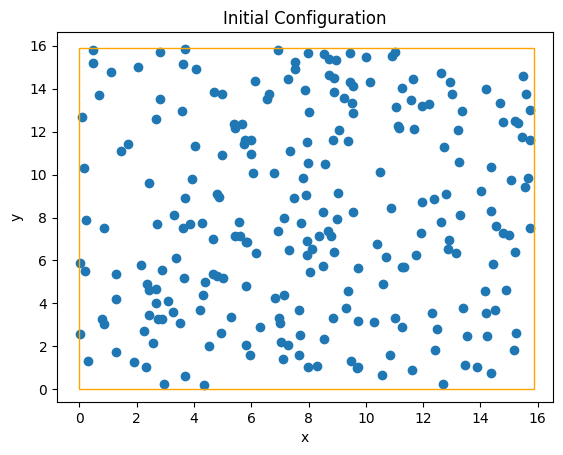
\includegraphics[width=.6\linewidth]{images/Start.png}
    \caption{}
    \label{fig:start}
\end{figure}
\noindent In the following Figure, we present the final configurations observed at each temperature. These configurations offer a comprehensive depiction of the optimal system's structural organisation.
\begin{figure}[H]
    \centering
    \begin{subfigure}{0.495\linewidth}
        \centering
        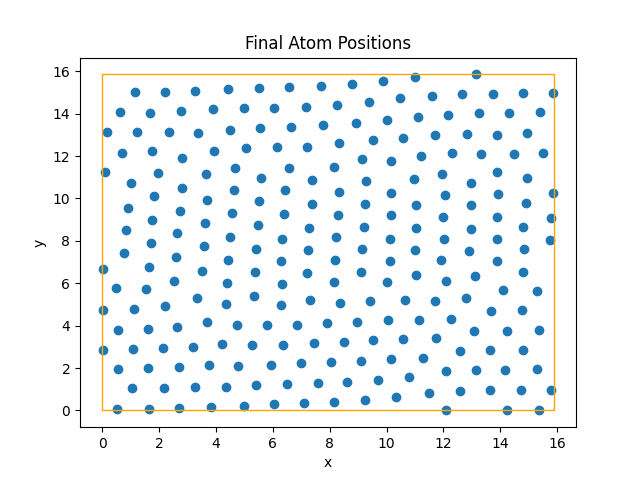
\includegraphics[width=\textwidth]{images/Final0.5.png}
        \caption{$T=0.5$}
    \end{subfigure}
    \hfill
    \begin{subfigure}{0.495\linewidth}
        \centering
        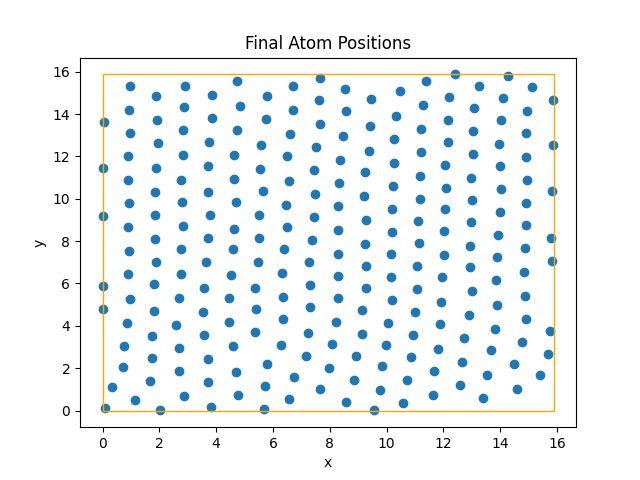
\includegraphics[width=\textwidth]{images/Final1.png}
        \caption{$T=1$}
    \end{subfigure}
\end{figure}
\begin{figure}[H]
    \begin{subfigure}{0.495\textwidth}
        \centering
        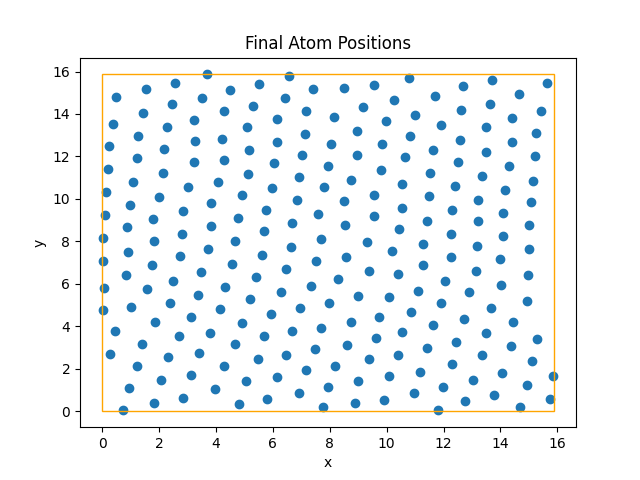
\includegraphics[width=\textwidth]{images/Final1.5.png}
        \caption{$T=1.5$}
    \end{subfigure}
    \hfill
    \begin{subfigure}{0.495\textwidth}
        \centering
        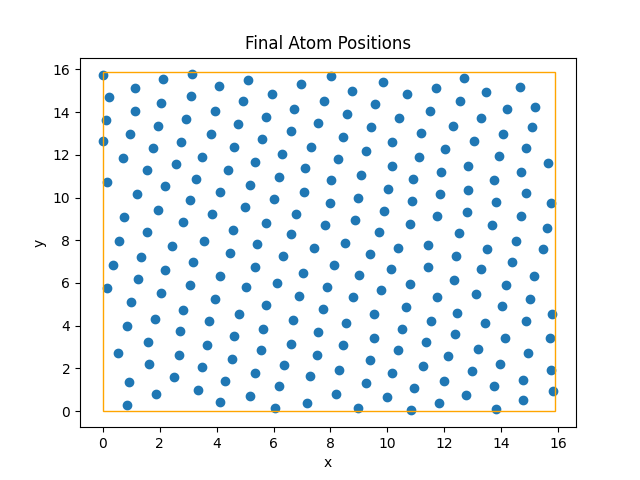
\includegraphics[width=\textwidth]{images/Final2.png}
        \caption{$T=2$}
    \end{subfigure}
    \medskip
    \begin{subfigure}{0.495\textwidth}
        \centering
        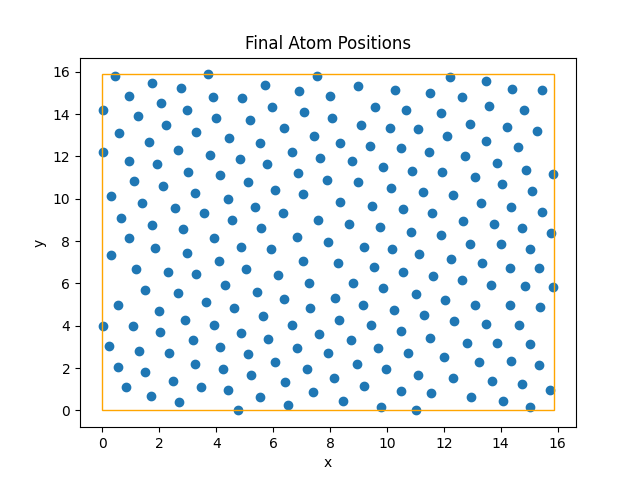
\includegraphics[width=\textwidth]{images/Final2.5.png}
        \caption{$T=2.5$}
    \end{subfigure}
    \hfill
    \begin{subfigure}{0.495\textwidth}
        \centering
        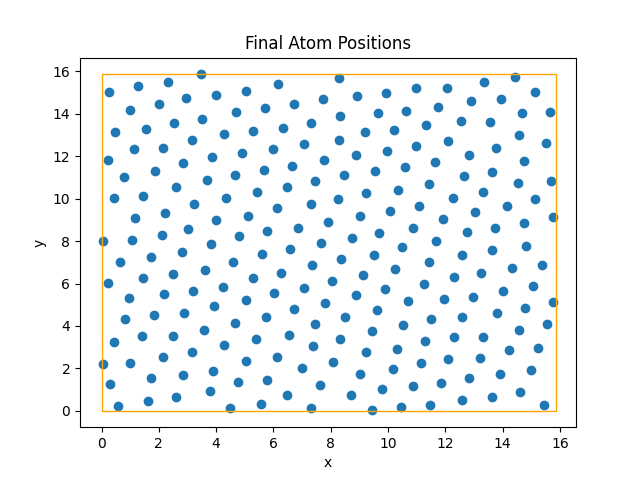
\includegraphics[width=\textwidth]{images/Final3.png}
        \caption{$T=3$}
    \end{subfigure}
    
    \caption{Final atom configurations}
\end{figure}
\noindent We can observe that the final configuration exhibits a higher degree of structural order, resembling a more closely packed crystal lattice.\\\\
We now present the radial distribution function corresponding to each temperature. This function offers valuable insights into the spatial arrangement of atoms.
\begin{figure}[H]
    \centering
    \begin{subfigure}{0.495\linewidth}
        \centering
        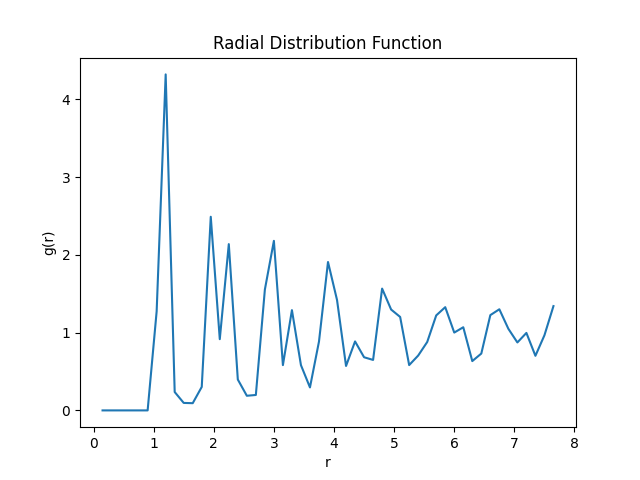
\includegraphics[width=\textwidth]{images/Radial0.5.png}
        \caption{$T=0.5$}
    \end{subfigure}
    \hfill
    \begin{subfigure}{0.495\linewidth}
        \centering
        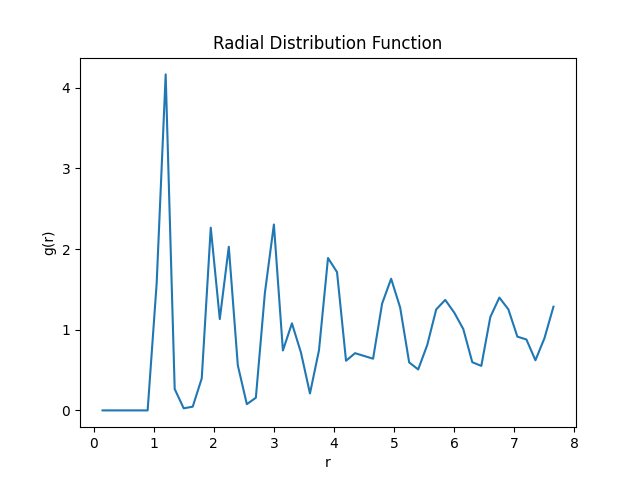
\includegraphics[width=\textwidth]{images/Radial1.png}
        \caption{$T=1$}
    \end{subfigure}
\end{figure}
\begin{figure}[H]
    \begin{subfigure}{0.495\textwidth}
        \centering
        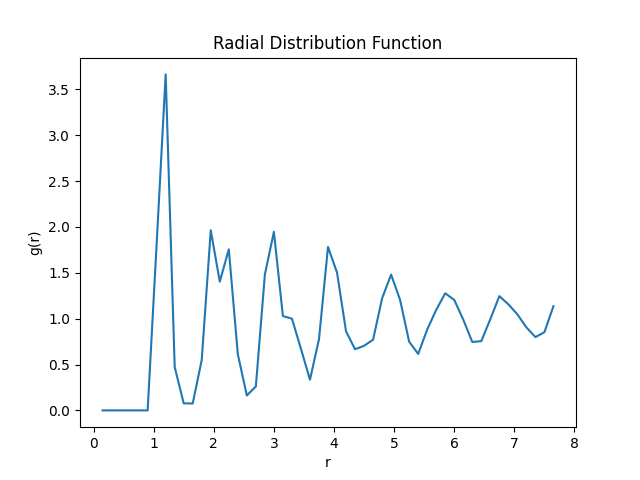
\includegraphics[width=\textwidth]{images/Radial1.5.png}
        \caption{$T=1.5$}
    \end{subfigure}
    \hfill
    \begin{subfigure}{0.495\textwidth}
        \centering
        \includegraphics[width=\textwidth]{images/radial2.png}
        \caption{$T=2$}
    \end{subfigure}
    \medskip
    \begin{subfigure}{0.495\textwidth}
        \centering
        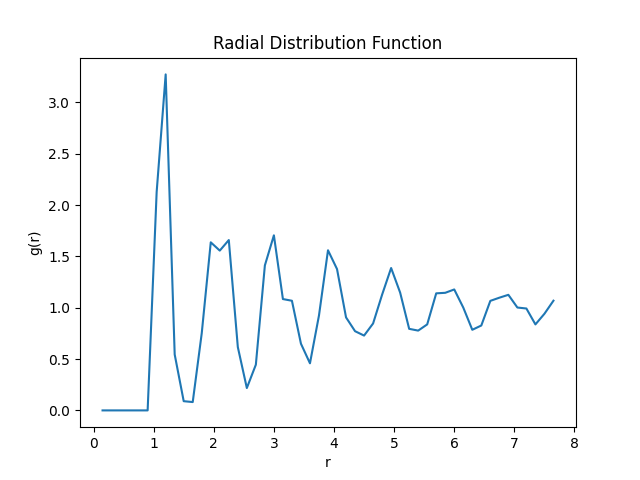
\includegraphics[width=\textwidth]{images/Radial2.5.png}
        \caption{$T=2.5$}
    \end{subfigure}
    \hfill
    \begin{subfigure}{0.495\textwidth}
        \centering
        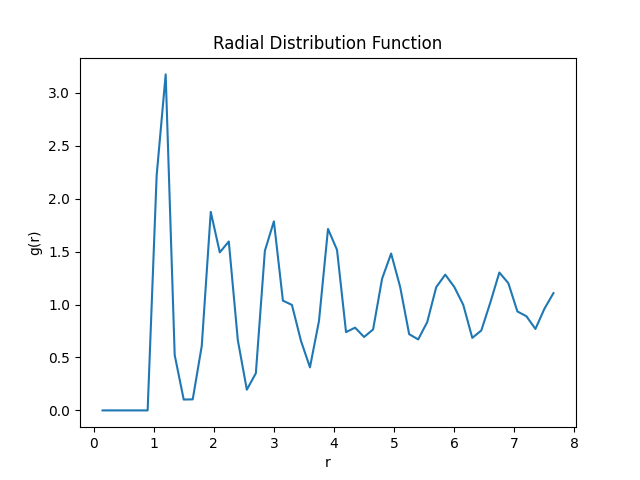
\includegraphics[width=\textwidth]{images/Radial3.png}
        \caption{$T=3$}
    \end{subfigure}
    
    \caption{Radial distribution function at various temperatures}
\end{figure}
\noindent Finally, we compare the radial distribution function depicted in \autoref{fig:radial} at two distinct temperatures. This comparative analysis enables us to discern how thermal variations affect the spatial distribution of particles within the system
\begin{figure}[H]
    \centering
    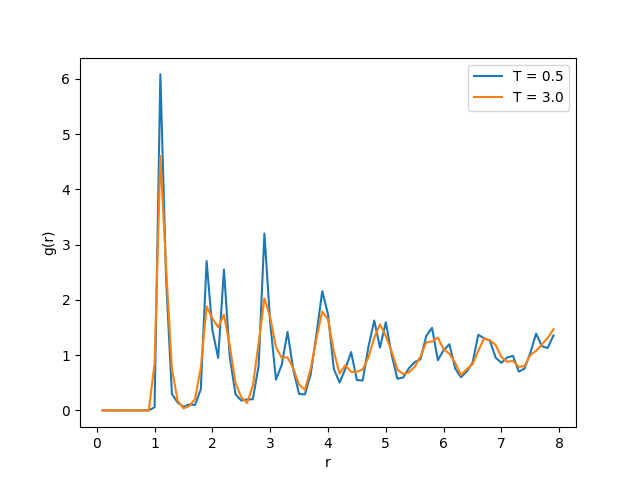
\includegraphics[width=.6\linewidth]{images/RadialComparison.png}
    \caption{Comparing radial distribution function at different temperatures}
    \label{fig:radial}
\end{figure}
\section{Conclusions}
In \autoref{tab:1}, we present the computed results of the average energy per atom and standard deviation.
\begin{table}[H]
    \centering
    \begin{tabular}{|c|c|c|}
        \hline
        $T$& $E^*$ [kJ] & Standard deviation \\\hline\hline
        0.5 & 1.152 e9 & 1.183 e9 \\\hline
        1 & 1.161 e9 & 1.209 e9 \\\hline
        1.5 & 1.235 e9 & 1.314 e9 \\\hline
        2 & 1.247 e9 & 1.312 e9 \\\hline
        2.5 & 1.335 e9 & 1.437 e9 \\\hline
        3 & 1.349 e9 & 1.442 e9 \\\hline
    \end{tabular}
    \caption{Results at different temperatures}
    \label{tab:1}
\end{table}
\end{document}
